% Compile twice!
% With the current MiKTeX, you need to install the beamer, and the translator packages directly form the package manager!

% Uncomment these to get the presentation form
%\documentclass{beamer}
%\geometry{paperwidth=200mm,paperheight=200mm, top=0in, bottom=0.2in, left=0.2in, right=0.2in}

% Uncomment these, and comment the 2 lines above, to get a paper-type article
\documentclass[10pt]{article}
\usepackage{geometry}
%\geometry{top=0.2in, bottom=0.2in, left=0.2in, right=0.2in}
\usepackage{beamerarticle}
\renewcommand{\\}{\par\noindent}
\setbeamertemplate{note page}[plain]

% Half A4 geometry
%\geometry{paperwidth=105mm,paperheight=297mm,top=0.2in, bottom=0.2in, left=0.2in, right=0.2in}

% "1/3" A4 geometry
%\geometry{paperwidth=105mm,paperheight=455mm,top=0.1in, bottom=0.1in, left=0.1in, right=0.1in}

% "1/6" A4 geometry
\geometry{paperwidth=105mm,paperheight=891mm,top=0.1in, bottom=0.1in, left=0.1in, right=0.1in}

% "1/5" A4 geometry
%\geometry{paperwidth=105mm,paperheight=740mm,top=0.1in, bottom=0.1in, left=0.1in, right=0.1in}

% "1/4" A4 geometry
%\geometry{paperwidth=105mm,paperheight=594mm,top=0.1in, bottom=0.1in, left=0.1in, right=0.1in}

% Uncomment these, to put more than one slide / page into a generated page.
%\usepackage{pgfpages}
% Choose one
%\pgfpagesuselayout{2 on 1}[a4paper]
%\pgfpagesuselayout{4 on 1}[a4paper]
%\pgfpagesuselayout{8 on 1}[a4paper]

% Compile twice!
% With the current MiKTeX, you need to install the beamer, and the translator packages directly form the package manager!

% Uncomment these to get the presentation form
\documentclass{beamer}
\geometry{paperwidth=170mm,paperheight=170mm}

% Uncomment these, and comment the 2 lines above, to get a paper-type article
%\documentclass[10pt]{article}
%\usepackage{beamerarticle}
%\renewcommand{\\}{\par\noindent}
%\setbeamertemplate{note page}[plain]

% Uncomment these, to put more than one slide / page into a generated page.
%\usepackage{pgfpages}
% Choose one
%\pgfpagesuselayout{4 on 1}[a4paper]
%\pgfpagesuselayout{8 on 1}[a4paper]


\usepackage{tikz}
\usetikzlibrary{shapes,arrows}

\usepackage[T1]{fontenc}
\usepackage{amsfonts}
\usepackage{amsmath}
\usepackage[utf8]{inputenc}
\usepackage{booktabs}
\usepackage{array}
\usepackage{arydshln}

% Beamer theme
\usetheme{boxes}

% tikz settings for the flowchart(s)

\tikzstyle{decision} = [diamond, minimum width=3cm, minimum height=1cm, text centered, draw=black, fill=green!15]
\tikzstyle{block} = [rectangle, draw, fill=blue!15, text width=20em, text centered, minimum height=1em]
    
\tikzstyle{line} = [draw, -latex']
\tikzstyle{cloud} = [draw, ellipse,fill=red!20, node distance=3cm,
    minimum height=2em]
\tikzstyle{arrow} = [thick,->,>=stealth]

\newcolumntype{C}[1]{>{\centering\let\newline\\\arraybackslash\hspace{0pt}}m{#1}}
\renewcommand{\arraystretch}{1.2}

\setlength\dashlinedash{0.2pt}
\setlength\dashlinegap{1.5pt}
\setlength\arrayrulewidth{0.3pt}

\begin{document}

\begin{frame}[plain]
\begin{beamercolorbox}[center]{title}
    {\Huge A Számítástudomány Alapjai I}
    \bigskip
\end{beamercolorbox}
\end{frame}

\begin{frame}
\begin{block}{}
\underline{\textbf{A kisbetűs szövegek (LaTeX-ben tiny), (Ha nincs előttük (S) jelzés, akkor lemaradt)}}\\
\underline{\textbf{a saját értelmezést jelentik, és egyáltalán nem garantált hogy jók!}}
\end{block}
\end{frame}

% --------------------  LOGIKA --------------------

\begin{frame}[plain]
\begin{beamercolorbox}[center]{title}
    {\Huge Logika}
    \medskip
\end{beamercolorbox}
\end{frame}

\begin{frame}

\begin{block}{(Ítélet) változók, Logikai szimbólumok, Elválasztó szimbólumok, Logikai formula}
\bigskip
\textbf{(Ítélet) változók:} $p_1, p_2, ...$\\
\hspace{1ex} \textbf{Jel: } $Var = \{p_1, p_2, ...\}$\\
\bigskip
\textbf{Logikai szimbólumok:} ${\neg}, {\land}, {\lor}, {\Rightarrow}, {\iff}.$\\
\bigskip
\textbf{Elválasztó szimbólumok:} $(, )$\\
\bigskip
\textbf{Logikai Formula:} Minden változó formula, továbbá ha $A, B$ formula, akkor:\\
\textbf{${\neg}A, (A \land B), (A \lor B), (A \Rightarrow B), (A \iff B)$} is formula.\\
\bigskip
Legyen $Form$ az összes formula halmaza.

\end{block}

\begin{block}{Megj}
\textbf{Precedencia:}\\ 
\bigskip
$1. {\neg}, 2. {\land}, 3. {\lor}$\\
\bigskip
$A \Rightarrow B \equiv {\neg}A \lor B$\\
$(A \iff B) \equiv (A \Rightarrow B) \land (B \Rightarrow A) \equiv ({\neg}A \lor B) \land ({\neg}B \lor A)$\\
\bigskip
(Az $\equiv$ jel itt a jobb elválasztást szolgálja, de egyébként alapból használható ugyanarra mint az $\iff$ jel!)

\end{block}

\end{frame}

\begin{frame}

\begin{block}{Tétel: Minden formula egyértelműen olvasható}
F formulára a következő állítások közül pontosan egy teljesül:

\begin{enumerate}
\item F egy változó.
\item Pontosan egy G formulára $F = \neg G$
\item Pontosan egy G és pontosan egy H formuláta $F = (G \land H)$
\item Pontosan egy G és pontosan egy H formulára $F = (G \lor H)$
\end{enumerate}

\end{block}

\end{frame}

\begin{frame}

\begin{block}{Részformula, Közvetlen részformula}
Ha $F$ és formulákra  $f = G_1GG_2$, alkalmas $G_1, G_2, E(G)$ szavakra, ($G_1, G_2$ üres szavak is lehetnek!)\\
akkor $G$ \textbf{részformulája} $F$-nek.\\
\bigskip
A tétel 2-4 pontjában szereplő $G$ és $H$ \textbf{közvetlen részformulái} $F$-nek.

\end{block}

\end{frame}

\begin{frame}

\begin{block}{Hozzárendelés}
Egy $\mathcal{A} : Var \rightarrow \{0, 1\}$ leképzést \textbf{hozzárendelésnek} nevezünk.\\
{\tiny (S) Ítéletváltozóhoz (Var az összes ítéletváltozó halmaza) hozzárendelünk elemet a {0, 1} halmazból. Kb értékadás. (kb függvény)}\\
\bigskip
$\mathcal{A} : Form \rightarrow \{0, 1\}$ kiterjesztéshez legyen $F$ formula.\\
{\tiny (S) Ugyan az, csak formulának adunk értéket.}\\
\bigskip
\begin{enumerate}
\item Ha $F = p$ valamely $p \in Var$ esetén, akkor $\mathcal{A}(F) = \mathcal{A}(p)$.\\
{\tiny (S) Ha F formula értéke mindíg ugyan az mint egy tetszőleges p ítéletváltozó értéke, akkor hozzárendelés után is megegyezik az értékük. Kb mint monotonitás. }\\
\bigskip
\item Ha $F = {\neg}G$ akkor:\\
\medskip
$\mathcal{A}(F)$ = $
\begin{cases}
1 &$ ha $\mathcal{A}(G) = 0\\
0 &$ ha $\mathcal{A}(G) = 1\\
\end{cases}
$
\bigskip
\item Ha $F = G \lor H$ akkor:\\ 
\medskip
$\mathcal{A}(F)$ = $
\begin{cases}
1 &$ ha $\mathcal{A}(G) = 1$ vagy $\mathcal{A}(H) = 1\\
0 &$ különben$\\
\end{cases}
$
\bigskip
\item Ha $F = G \land H$ akkor:\\
\medskip
$\mathcal{A}(F)$ = $
\begin{cases}
1 &$ ha $\mathcal{A}(G) = 1$ és $\mathcal{A}(H) = 1\\
0 &$ különben$\\
\end{cases}
$
\end{enumerate}

\end{block}

\end{frame}

\begin{frame}

\begin{block}{Formula modellje, Kielégíthető, Tautológia, Kielégíthetetlen}
Legyen $F$ formula, Legyen $\mathcal{A}$ egy hozzárendelés.s Ekkor\\
\bigskip
Ha $\mathcal{A}(F) = 1$, akkor ezt a tényt $\mathcal{A} \models F$-fel jelöljük, és azt mondjuk, hogy $\mathcal{A}$ \textbf{kielégíti} $F$-et, vagy hogy $\mathcal{A}$ \underline{\textbf{modellje}} $F$-nek.\\
{\tiny (S) Mint egy függvén kb. F formulához hozzárendelünk egy értéket, és ha ez 1)}\\
\bigskip
Ha $F$-nek van modellje, akkor azt mondjuk, hogy $F$ \underline{\textbf{kielégíthető}}.\\
\bigskip
Ha minden $\mathcal{A}$ hozzárendelés esetén $\mathcal{A} \models F$, akkor $F$ \underline{\textbf{tautológia}} (vagy másképpen érvényes).\\
Jele: $\models F$.\\
\bigskip
Ha $F$-nek nincs modellje, akkor azt mondjuk, hogy $F$ \underline{\textbf{kielégíthetetlen}}.\\
\bigskip
Legyen $\Sigma$ formulák egy halmaza. Ha valamely $\mathcal{A}$ hozzárendelés esetén minden $F \in \Sigma$-re $\mathcal{A} \models F$, akkor ezen tényt $\mathcal{A} \models \Sigma$-val jelöljük, és azt mondjuk, hogy $\mathcal{A}$ kielégíti $\Sigma$-t vagy, hogy $\mathcal{A}$ modellje $\Sigma$-nak.\\
{\tiny (S) Ha van egy olyan $\mathcal{A}$ hozzárendelésünk, amire a $\Sigma$ halmaz összes formulája igazat ad.}\\
\bigskip
Ha $\Sigma$-nak van modellje, akkor azt mondjuk, hogy $\Sigma$ kielégíthető.
\end{block}

\end{frame}

\begin{frame}

\begin{block}{Tétel: Az ítéletkalkulus kompaktsági tétele}
Egy formulahalmaz akkor és csak akkor elégíthető ki, ha minden véges részhalmaza kielégíthető.

\end{block}

\end{frame}

\begin{frame}

\begin{block}{K változós igazságtábla}
Tetszőleges $k \in \mathbb{N}$ esetén az IT: $\{0, 1\}^k \rightarrow \{0, 1\}$ leképzést \textbf{$k$ változós igazságtáblának (Boole függvény)} nevezzük.
\end{block}

\begin{block}{Igazságtáblák:}
\begin{table}[h!]
\centering
Negáció (unér művelet)\\
\bigskip
\begin{tabular}{@{}C{3em}C{3em}@{}}
\toprule
\textbf{$A$} & \textbf{${\neg}A$} \\
\hline
i & h\\
\hdashline
h & i\\
\toprule
\end{tabular}
\end{table}
\bigskip

\begin{table}[h!]
\centering
A többi művelet\\
\bigskip
\begin{tabular}{C{1em}C{1em}rC{4.4em}C{4.4em}C{4.4em}C{4.4em}}
\toprule
\textbf{$A$} & \textbf{$B$} & \textbf{$|$} & \textbf{$A \land B$} & \textbf{$A \lor B$} & \textbf{$A \Rightarrow B$} & \textbf{$A \iff B$} \\
\hline
i & i & | & i & i & i & i\\
\hdashline
i & h & | & h & i & h & h\\
\hdashline
h & i & | & h & i & i & h\\
\hdashline
h & h & | & h & h & i & i\\
\toprule
\end{tabular}
\end{table}

\end{block}

\end{frame}

%\begin{frame}
%\begin{block}{Def: {Az $F$ formula által meghatározott Igazság tábla}
%\textbf{Az $F$ formula által meghatározott $IT_F$ igazságtábla:}\\
%ha $p_1, ..., p_n$ az $F$ változói és $x_1, ..., x_n \in \{0, 1\}$, akkor\\
%$IT_F(x_1, ..., x_n) = A(F)$, ahol $A(p_j) = x_j, 1 \leq j \leq n$.
%\end{block}
%\end{frame}

\begin{frame}

\begin{block}{Def: Adekvát halmaz}
A ${\neg}, {\land}, {\lor}, \rightarrow$ műveleti jelek C halmaza \textbf{adekvát}, ha\\
$IT: \{0, 1\}^k \rightarrow \{0, 1\}, k \geq 1$ igazságtábla esetén van olyan $F \in Form$, hogy\\
\begin{enumerate}
\item $F$-ben csak $C$-beli műveletei jelek szerepelhetnek,
\item $IT = IT_F$.
\end{enumerate} 
\end{block}
\bigskip

\begin{block}{Tétel: Adekvát halmazok}
$\{\neg, \lor, \land\}, \{\neg, \lor\}, \{\neg, \land\}$ adekvát (azaz bármilyen formula leírható ezekkel), $\{\lor, \land\}$ nem adekvát.
\end{block}

\end{frame}

\begin{frame}
\begin{block}{Def.: Logikai következmény}
Legyen $\Sigma \subseteq Form$ és $F \in Form$.\\
Azt mondjuk, hogy $F$ \underline{\textbf{logikai következménye}} $\Sigma$-nak, (jele: $\Sigma \models F$),\\
ha minden $\mathcal{A}$ hozzárendelés esetén valahányszor $\mathcal{A} \models \Sigma$, mindannyiszor $\mathcal{A} \models F$ is teljesül.\\
{\tiny (S) logikai következmény egyenlő a $A \Rightarrow B$ boole függvénnyel, ha kikötjük, hogy A csak igaz lehet. (Mivel az alap Boole függvényben ha $A$ hamis, akkor az eredmény igaz!)}
\end{block}
\medskip
\begin{block}{Ész}
\begin{enumerate}
\item $F$ akkor és csak akkor érvényes (tautológia), ha $\emptyset \models F$. Tehát $\models F$. és $\emptyset \models F$ ugyanazt jelenti.\\
{\tiny (S) Kb mintha csak rövidítva lenne}\\
\item Ha $F$ érvényes, akkor minden $\Sigma$-ra $\Sigma \models F$\\
{\tiny (S) Igen, mert bármikor amikor $\Sigma$ összes formulája egyszerre igazat ad vissza $F$ is igaz (mivel F tautológia).}\\
\item Ha $F \in \Sigma$, akkor $\Sigma \models F$\\
{\tiny (S) Igen, mert bármikor amikor $\Sigma$ összes formulája egyszerre igazat ad vissza $F$ garantáltan igaz (Persze F lehet többször igaz).}\\
\item Minden $F$-re $\downarrow \models F$.\\
{\tiny (S) Ugyan az mint az előbb, csak mivel $\downarrow$ sose igaz, ezért a feltétel mindíg teljesül.}\\
\item Minden $F$-re és $G$-re $F \models G$ akkor és csak akkor teljesül, ha $F \rightarrow G$ érvényes (= tautológia).\\
{\tiny (S) A $\rightarrow$ boole függvény, ha $F$ hamis, akkor igazat ad vissza mindíg. (Ez nem probléma, mert az $F$ hamis rész, a logikai következménynény definícióban nem számít)}\\
\item (Modus Ponens, röviden MP) Minden $\Sigma$-ra, $F$-re és $G$-re $\Sigma \cup \{F, F \rightarrow G\} \models \Sigma \cup \{G\}$\\
{\tiny (S) 3. 5. 8. pontok összekombinálása eggyé.}\\
\item (Monotonitás) Ha $\Sigma \subseteq {\Sigma}_1$, akkor minden $F$-re, ha $\Sigma \models F$, akkor ${\Sigma}_1 \models F$.\\
{\tiny (S) Persze, ${\Sigma}_1$ részhalmaz.}\\
\item (Következmény) Minden $\Sigma$-ra, F-re, G-re $\Sigma \models F \rightarrow G$ akkor és csak akkor teljesül, ha $\Sigma \cup \{F\} \models G$.\\
{\tiny (S) Persze, mert ha $F$ hamis, akkor a $\Sigma$ halmaz gyakorlatilag hamisat ad vissza, mert egy eleme hamis (ekkor nem számít), ha pedig $F$ igaz (ettől még nem muszály $\Sigma$-nak igazat visszaadnia, ha esetleg ilyenkor is hamis, attól még ugyanúgy működik, pl $\Sigma$ $\downarrow$, ekkor logikai következmény lesz akkor is, ha $F \rightarrow G$ hamisat ad vissza. (Lásd 4. pont)), akkor meg kell nézni $G$-t, viszont ha ilyenkor $G$ hamis, akkor nem logikai következmény.}
\end{enumerate}
\end{block}

\end{frame}

\begin{frame}

\begin{block}{tétel: Ekvivalens állítások formulákra}
Legyenek $F, F_1, ... , F_n$ tetszőleges formulák, ekkor a következő állítások equivalensek:
\begin{enumerate}
\item $\{F_1, ... , F_n\} \models F$
\item $F_1 \land ... \land F_n \rightarrow F$ tautológia
\item $F_1 \land ... \land F_n \land \neg F$ kielégíthetetlen.
\end{enumerate}
\end{block}

\end{frame}

\begin{frame}

\begin{block}{Ekvivalens formulák}
Az igaz és hamis szabályok:\\
${\neg}\downarrow \equiv \uparrow$\\
${\neg}\uparrow \equiv \downarrow$\\
$F \land \downarrow \equiv \downarrow$, és $\downarrow \land F \equiv \downarrow$\\
$F \land \uparrow \equiv F$, és $\uparrow \land F \equiv F$\\
$F \lor \uparrow \equiv \uparrow$, és $\uparrow \lor F \equiv \uparrow$\\
$F \lor \downarrow \equiv F$, és $\downarrow \lor F \equiv F$\\
\smallskip
Kontrapozíció (Modus Tollens):\\
$A \Rightarrow B \iff {\neg}B \Rightarrow {\neg}A$\\
\smallskip
A de Morgan szabályok:\\
${\neg}(F \land G) \equiv {\neg}F \lor {\neg}G$\\
${\neg}(F \lor G) \equiv {\neg}F \land {\neg}G$\\
\smallskip
Az idempotencia szabályai:\\
$F \land F \equiv F$\\
$F \lor F \equiv F$\\
\smallskip
A kommutativitás szabályai:\\
$F \land G \equiv G \land F$\\
$F \lor G \equiv G \lor F$\\
\smallskip
Az asszociativitás szabályai:\\
$(F \land G) \land H \equiv F \land (G \land H)$\\
$(F \lor G) \lor H \equiv F \lor (G \lor H)$\\
\smallskip
Az adszorpció szabályai:\\
$F \land (F \lor G) \equiv F$\\
$F \lor (F \land G) \equiv F$\\
\smallskip
A disztributivitás szabályai:\\
$F \land (G \lor H) \equiv (F \land G) \lor (F \land H)$\\
$F \lor (G \land H) \equiv (F \lor G) \land (F \lor H)$\\
\smallskip
A dupla negáció szabálya:\\
${\neg}{\neg}F \equiv F$
\end{block}

\end{frame}

\begin{frame}

\begin{block}{Lemma: Helyettesítési Lemma}
Legyenek $F, G, H$ formulák úgy, hogy $F \equiv G$ és $F$ a $H$ részformulája.\\
Ha $H[F/G]$ azt a formulát jelöli, amelyben $F$ valamely előfordulását helyettesítettük $G$-vel, akkor
$$H \equiv H[F/G]$$
\end{block}

\end{frame}

\begin{frame}

\begin{block}{Def.: Literál}
Egy $F$ formulát \textbf{pozitíb literálnak} nevezünk, ha $F = p$, és \textbf{negatív literálnak}, ha $F = {\neg}o$, ahol $p$ változó.
\end{block}

\begin{block}{Def.: Konjunktív, diszjunktív normálforma}
Egy $F$ formula \textbf{Konjunktív normálforma}, ha:\\
$$F = \bigwedge_{i = 1}^n (\bigvee_{j = 1}^{m_i} l_{i, j}))$$\\
Egy $F$ formula \textbf{Diszjunktív normálforma}, ha:\\
$$F = \bigvee_{i = 1}^n (\bigwedge_{j = 1}^{m_i} l_{i, j}))$$\\
ahol $l_{i, j}$-k literálok.
\end{block}

\end{frame}

\begin{frame}

\begin{block}{Tétel: Konjunktív és diszjunktív normálforma létezése}
Minden $F$ Formulához létezik vele logikailag ekvivalens konjunktív és diszjunktív normálforma.
\end{block}

\begin{block}{Bizonyítás}
Konjunktív:
\begin{enumerate}
	\item (Negáció bevitele.) Amíg lehetséges, helyettesítsük $F$-ben a
	\begin{itemize}
		\item $\neg \neg G$ alakú részformulákat $G$-vel,
		\item $\neg (G \land H)$ alakú részformulákat $\neg G \lor \neg H$-val,
		\item $\neg (G \lor H)$ alakú részformulákat $\neg G \land \neg H$-val.
	\end{itemize}
	\item Amíg lehetséges, helyettesítsük $F$-ben a
	\begin{itemize}
		\item $F \lor (G \land H)$ alakú részformulákat $(F \lor G) \land (F \lor H)$-val,
		\item $(F \land G) \lor H$ alakú részformulákat $(F \lor H) \land (G \lor H)$-val.
	\end{itemize}
\end{enumerate}
\bigskip
Diszjunktív:
\begin{enumerate}
	\item Ugyanaz mint a konjunktív normálforma esetén.
	\item Amíg lehetséges, helyettesítsük $F$-ben a
	\begin{itemize}
		\item $F \land (G \lor H)$ alakú részformulákat $(F \land G) \lor (F \land H)$-val,
		\item $(F \lor G) \land H$ alakú részformulákat $(F \land H) \lor (G \land H)$-val.
	\end{itemize}
\end{enumerate}
\end{block}

\end{frame}

\begin{frame}

\begin{block}{Def.: Elmélet}
Legyen $\Sigma$ egy formulahalmaz, ekkor:\\
\smallskip
$Th({\Sigma}) = \{F | \Sigma \models F\}$ a \textbf{$\Sigma$ által generált elmélet}.\\
($Th({\Sigma})$ a $\Sigma$ összes logikai következménye).
\end{block}

\begin{block}{Def.: Levezetés, bizonyítható formula}
Ha $\Sigma$ formulák egy halmaza, akkor az $F_1, ... F_n$ formulák sorozatát a \textbf{$\Sigma$-ból történő ($\Sigma$ feletti) bizonyításnak levezetésnek)} nevezünk, ha minden $1 \leq i \leq n$ esetén az aláőbbi feltételek valamelyike teljesül:\\
\begin{enumerate}
\item $F_i \in \Sigma$
\item $F_i$ tautológia
\item van olyan $k, l < i$, hogy $F_l = F_k \rightarrow F_i$
\end{enumerate}
\bigskip
Egy $F$ formula \textbf{bizonyítható (levezethető)} $\Sigma$-ból, ha van olyan $\Sigma$ feletti $F_1, ..., F_n$ bizonyítás, hogy $F_n = F$.\\
\bigskip
\textbf{Jel.: $\Sigma \vdash F$}
\end{block}

\end{frame}

\begin{frame}

\begin{block}{Def.: Modus Ponens}
Ha valamely $A$ hozzáredelésre teljesül, hogy:\\
$A \models F$ és $A \models F \rightarrow G$, akkor $A \models G$.
\end{block}

\begin{block}{Def.: Modus Tollens (Kontrapozíció)}
$A \Rightarrow B \iff {\neg}B \Rightarrow {\neg}A$.
\end{block}

\begin{block}{Def.: Indirekt Bizonyítás}
Tetszőleges $\Sigma$ formulahalmaz esetén $\Sigma \vdash F \rightarrow G$ akkor és csak akkor teljesül, ha:\\
$\Sigma \cup \{F\} \vdash G$.
\end{block}

\end{frame}

\begin{frame}

\begin{block}{Tétel: Dedukció tétel}
Tetszőleges $\Sigma$ formulahalmaz esetén $\Sigma \vdash F \rightarrow G$ akkor és csak akkor teljesül, ha $\Sigma \cup \{F\} \vdash G$.
\end{block}

\begin{block}{Tétel: Dichotómia tétel}
Tetszőleges $\Sigma$ formulahalmaz esetén, ha $\Sigma \cup \{F\} \vdash$ (levezethető) $G$ és $\Sigma \cup \{\neg F\} \vdash G$, akkor $\Sigma \vdash G$.\\
("Az $F$ Formula nem szól bele").
\end{block}

\begin{block}{Tétel: Helyességi tétel}
Tetszőleges $\Sigma$ és $F$ esetén, ha $\Sigma \vdash F$, akkor $\Sigma \models F$.\\
(Helyes, ha csak az elélethez tartozó formulákat lehet bizonyítani.)
\end{block}

\begin{block}{Tétel: Teljességi tétel}
Minden $\Sigma$-ra és $F$-re, ha $\Sigma \models F$, akkor $\Sigma \vdash F$.\\
(Teljes, ha minden, az elmélethez tartozó formulát be lehet bizonyítani.)
\end{block}

\begin{block}{Tétel: Konzisztencia tétel}
Tetszőleges formulahalmaz, akkor és csak akkor konzisztens, ha kielégíthető.\\
(Konzisztens, ha nem vezethető le belőle a $\downarrow$.)
\end{block}

\end{frame}

% --------------------  PREDIKÁTUMKALKULUS (1-RENDŰ LOGIKA) --------------------

\begin{frame}[plain]
\begin{beamercolorbox}[center]{title}
    {\Huge Predikátumkalkulus (1-Rendű Logika)}
\end{beamercolorbox}
\end{frame}

\begin{frame}

\begin{block}{$A$ feletti n változó predikátum}
\textbf{$A$ feletti n változó predikátum} a következő függvény:\\
$p \rightarrow A^n \rightarrow \{0, 1\}$
\end{block}

\begin{block}{Az $L$ elsőrendű nyelv szimbólumai}
TODO
\end{block}

\begin{block}{Az $L$ elsőrendű nyelv formulái}
TODO
\end{block}

\begin{block}{Kötött, szabad változó, nyílt, zárt formula}
TODO
\end{block}

\begin{block}{Az elsőrendű nyelv szemantikája}
TODO
\end{block}

\end{frame}

% --------------------  GRÁFELMÉLET --------------------

\begin{frame}[plain]
\begin{beamercolorbox}[center]{title}
    {\Huge Gráfelmélet}
\end{beamercolorbox}
\end{frame}


\begin{frame}

\begin{block}{Gráf}
A $G = (V, E, {\phi})$ hármast \textbf{(irányítatlan) gráfnak} nevezzük, ha $V, E$ halmazok, $V \neq \emptyset, V \cap E = \emptyset$, és $\phi : E \rightarrow [V]^2$.\\
\bigskip
$[V]^2 = \{ [a, b] | a, b \in V \}$, ahol $[a, b] = [b, a]$\\
\bigskip
\textbf{V}: pont-, csúcshalmaz. $V(G)$ $G$ pontjai, $v(G) = |V(G)| = \#V$ G pontjainak száma.\\
\bigskip
\textbf{E}: élhalmaz. $E(G)$ $G$ élei, $e(G) = |E(G)| = \#E$ G éleinek száma.\\
\bigskip
(E = Edge, V = Vertex)
\end{block}

\begin{block}{Ész}
\begin{enumerate}
\item $E = dmn({\phi})$
\item ${\phi}(e) = \{v_1, v_2\} \subseteq V$ minden $e \in E$-re.
\end{enumerate}
\end{block}

\end{frame}


\begin{frame}

\begin{block}{Egyéb definíciók}
\begin{itemize}
\item \textbf{Véges gráf:} Ha $V(G)$ és $E(G)$ is véges.
\item \textbf{Él végpontjai / él illeszkedése:}\\
$e \in E$ él végpontjai ($e$ illeszkedik $a$-ra, és $b$-re) ha $a, b \in V$ esetén ${\phi}(e) = [a, b]$
\item \textbf{Hurokél:} Ha a = b.
\item \textbf{Párhuzamos (többszörös él):} Ha $e, f \in E$, és ${\phi}(e) = {\phi}(f)$
\item \textbf{Szomszédos él:} Ha $e, f \in E$ és ${\phi}(e) = [a_1, a_2], {\phi}(f) = [b_1, b_2]$ esetén $\{a_1, a_2\} \cap \{b_1, b_2\} \neq \emptyset$
\item \textbf{Szomszédos csúcsok:} Ha $a_1, a_2 \in V$, és $a_1 \neq a_2$, és ${\exists}e \in E$, amire ${\phi}(e) = [a_1, a_2]$
\item \textbf{Csúcs foka:} A rá illeszkedő élek száma (huroknál 2), jelölés: \textbf{d(a)}
\item \textbf{Izolált csúcs:} $a$ csúcs izolált, ha d(a) = 0
\item \textbf{Egyszerű gráf:} Hurok és többszörös él nélküli gráf.
\item \textbf{Reguláris gráf:} A $G = (V, E)$ gráf \textbf{reguláris}, ha $d(a)$ értéke azonos minden $a \in V$-re, \textbf{n-reguláris}, ha ekkor $d(a) = n$ valamely $n \in \mathbb{N}$-re.
\end{itemize}
\end{block}

\end{frame}

\begin{frame}

\begin{block}{Tétel: Fokszám-Élszám}
Legyen $G = (V, E)$ (Gráf). Ekkor $G$-ben a páratlan fokú csúcsok száma páros.

\end{block}

\begin{block}{Bizonyítás}
$$\sum_{a \in V} d(a) = \sum_{d(a) \equiv 0 (mod 2)} d(a) + \sum_{d(a) \equiv 1 (mod 2)} d(a) \equiv 0 (mod 2)$$
amiből kapjuk, hogy $$\sum_{d(a) \equiv 1 (mod 2)} d(a) \equiv 0 (mod 2)$$.

\end{block}

\end{frame}

\begin{frame}

\begin{block}{Def.: Gráfok izomorfiája}
A $G = (V, E)$ és $G' = (V', E')$ gráf \textbf{izomorf},\\
ha létezik ${\pi} : V \rightarrow V'$, és $\rho : E \rightarrow E'$ bijekció úgy, hogy ha $a \in V$ és $e \in E$ illeszkedik $G$-ben $\iff$ ${\pi}(a)$ és ${\rho}(e)$ illeszkedik $G'$-ben.\\
\bigskip
A $G = (V, E)$ és $G' = (V', E')$ egyszerű gráf \textbf{izomorf}, ha létezik ${\pi} : V \rightarrow V'$ bijekció úgy, hogy $a, b \in V$ szomszédos $G$-ben $\iff$ ${\pi}(a)$ és ${\pi}(b)$ szomszédos G'-ben.\\
\bigskip
A $G = (V, E)$ egyszerű gráf \textbf{teljes gráf}, ha bármely két pontja szomszédos. \textbf{$K_n$} jelöli az \textbf{n} pontú teljes gráfot.
\end{block}

\begin{block}{Ész}
Ugyanannyi csússzámú teljes gráfok izomorfak.\\
\bigskip
$K_n$-nek $\frac{n(n - 1)}{2}$ éle van.
\end{block}
\end{frame}

\begin{frame}

\begin{block}{Def.: Páros Gráf}
A $G = (V, E, {\phi})$ hármast \textbf{páros gráfnak} nevezzük, ha $V = V' \cup V'', V' \cap V'' = \emptyset$, és $G$ minden élének egyik végpontja $V'$-ben, másik végpontja $V''$-ben van.\\
\medskip
($K_{3, 3}$ 6 pontú teljes páros gráf, $K_5$ 5 pontú teljes gráf.)
\end{block}
\begin{block}{Def.: Részgráf}
A $G' = (V', E', {\phi}')$ gráf a $G = (V, E, {\phi})$ gráf \textbf{részgráfja}, ha\\
$V' \subseteq V$ és $E' \subseteq E$, valamint ${\phi}'(e) = {\phi}(e)$ minden $e \in E'$-re.
\end{block}
\begin{block}{Def.: Telített Részgráf}
Ha a $G' = (V', E', {\phi}')$ gráf a $G = (V, E, {\phi})$ gráf részgráfja, és $E'$ mindazon $E$-beli elemeket tartalmazza, amelyek végpontjai $V'$-ben vannak, akkor $G'$-t \textbf{telített részgráfnak} nevezzük, vagy pontosabban \textbf{$V'$ által meghatározott telített részgráfnak.}
\end{block}
\begin{block}{Komplementer Gráf}
$\overline{G}$ an $n$-pontú egyszerű $G = (V, E)$ gráf \textbf{komplementer gráfja}, ha\\
\smallskip
$\overline{V}(G) = V(G)$ és\\
$E(\overline{G}) = E(K_n) \setminus E(G)$.
\end{block}

\end{frame}

\begin{frame}
\begin{block}{Zárt, Nyílt élsorozat (Séta)}
Legyen $k$ természetes szám.\\
\textbf{$k$ hosszú élsorozat (séta) $a_0$-ból $a_k$-ba} az\\
\smallskip
$[a_0, e_1, a_1, e_2, a_2, ..., e_k, a_k]$ sorozat, ha $a_0, a_1, ..., a_k \in V(G), e_1, e_2, ..., e_k \in E(G)$ és ${\phi}(e_i) = [a_{i - 1}, a_i]$ minden $i = 1, 2, ..., k$-ra.\\
\bigskip
\textbf{Út, Vonal:}\\
Egy élsorozat \textbf{út}, ha benne minden csúcs különböző és \textbf{vonal}, ha minden éle különboző.\\
\bigskip
\textbf{Zárt, Nyílt:}\\
Egy élsorozat \textbf{zárt}, ha $a_0 = a_k$ különben \textbf{nyílt}.\\
\bigskip
\textbf{Kör:}\\
\textbf{Kör} az a zárt élsorozat, melyben a többi csúcs egymástól és $a_0$-tól különbözik, és élei is mind különbözőek.\\
\bigskip
Út $\subset$ Vonal $\subset$ Séta\\
\medskip
Kör $\subset$ Zárt vonal $\subset$ Zárt séta
\end{block}
\begin{block}{Ész}
\begin{itemize}
\item Út és kör hossza az éleinek száma.
\item 0 hosszúságú séta út
\item út mindig vonal
\end{itemize}
\end{block}

\end{frame}

\begin{frame}
\begin{block}{Def.: Összeföggőség}
Egy gráf \textbf{összefüggő}, ha benne bármilyen két csúcs összeköthető sétával (következtetésképpen úttal is).
\end{block}
\begin{block}{Def.: Komponensek}
Legyen $\sim$ a következő ekvivalenciareláció (Reflexív, Tranzitív, Szimmetrikus):\\
\bigskip
$a_1, a_2 \in V(G)$ esetén $a_1 \sim a_2$, ha $a_1 = a_2$ vagy $a_1$ és $a_2$ között van út.\\
\bigskip
Az azonos osztályokba eső csúcsok által meghatározott telített részgráfok a $G$ gráf \textbf{(összefüggő) komponensei}, számuk \textbf{c(G)}.
\end{block}
\begin{block}{Ész}
\begin{itemize}
\item Különböző osztályokba eső csúcsok nem szomszédosak
\item Minden él hozzárendelhető egy komponenshez
\item Egy gráf összefüggő, ha egy komponense van
\end{itemize}
\end{block}
\end{frame}

\begin{frame}
\begin{block}{Def.: Fa}
Összefüggő körmentes gráf.
\end{block}
\end{frame}

\begin{frame}
\begin{block}{Tétel: Equivalens állítások fákra}
Egy $G$ egyszerű gráfra a következő állítások equivalensek:
\begin{enumerate}
\item $G$ Fa
\item $G$ Összefüggő, de bármely él elhagyásával kapott részgráf már nem összefüggő.
\item Ha $v, v'$ a $G$ különböző csúcsai, akkor pontosan egy út vezet $v$-ből $v'$be.
\item $G$-ben nincs kör, de bármely új él hozzáadásával kapott gráf már tartalmaz kört.
\end{enumerate}
\end{block}

\begin{block}{Tétel: Elsőfokú pontok}
Ha egy véges gráfban nincs kör, de van él, akkor van benne legalább két elsőfokú pont.
\end{block}
\end{frame}

\begin{frame} 
\begin{block}{Tétel: Ekvivalens állítások n-pontú fákra}
Egy $G$ egyszerű gráfra a következő álítások ekvivalensek:
\begin{enumerate}
\item $G$ fa.
\item $G$-ben nincs kör és $n - 1$ éle van.
\item $G$ összefüggő és $n - 1$ éle van.
\end{enumerate}
\end{block}

\begin{block}{Def.: Feszítőfa}
Az $F$ gráf a $G$ gráf \textbf{feszítőfája}, ha\\
$F$ részgráfja $G$-nek, $F$ fa és $V(T) = V(G)$.
\end{block}

\begin{block}{Tétel: Feszítőfa létezése}
Minden véges összefüggő $G$ gráfnak létezik feszítőfája.
\end{block}

\end{frame}

\begin{frame} 
\begin{block}{Tétel: Körök száma}
Egy véges összefüggő $G = (E, V)$ gráfban létezik \underline{legalább} $e(G) - v(G) + 1$ különböző kör.
\end{block}

\begin{block}{Bizonyítás}
A feszítőfa létezése téltel miatt ($\Rightarrow$) $\exists T$ feszítőfa, aminek $v(G) - 1$ éle van.\\
Legyen $K_f$ az a kör, ami $T \cup \{f\}$-ben van, ahol $f \in E(G) \setminus E(T)$\\
$T_G$ komplementerben legalább $e(G) - e(T) = e(G) - (v(G) - 1) = e(G) - v(G) - 1$ ilyen $f$ él van.\\
$\Rightarrow$ legalább $e(G) - v(G) + 1$ különbző kör.
\end{block}
\end{frame}

\begin{frame}
\begin{block}{Elvágó élhalmaz, vágás}
Legyen $G =  (V, E, {\phi})$ egy gráf, $v, w \in V$, és $V' \subseteq V$.\\
\bigskip
Ha minden $v$-ből $w$-be vezető út tartalmaz $V'$-beli csúcsot, akkor\\
\medskip
\textbf{$V'$ elvágja $v$-t, és $w$-t}.\\
\medskip
Ha $E' \subseteq E$ és minden $v$-ből $w$-be vezető út tartalmaz $E'$-beli élet, akkor\\
\medskip
\textbf{$E'$ elvágja $v$-t, és $w$-t}.\\
\bigskip
Ha $V'$, illetve $E'$ egy elemű, akkor \textbf{elvágó (szeparáló) pontról}, ill \textbf{elvágó (szeparáló) élről} beszélünk.\\
\bigskip
$E' \subseteq E$ \textbf{elvágó, (szeparáló) élhalmaz}, ha a $G' = (V, E \setminus E')$ több komponensből áll, mint $G$. (azaz vannak olyan csúcsok $G$-ben, amelyeket $E'$ elvág.)\\
\bigskip
$E' \subseteq E$ \textbf{vágás}, ha elvágó élhalmaz, de semelyik  valódi részhalmaza nem az.
\end{block}
\end{frame}

\begin{frame}
\begin{block}{Tétel: Vágások száma}
Egy véges összefüggő $G = (V, E)$ gráfban létezik legalább $v(G) - 1$ vágás.
\end{block}

\begin{block}{Bizonyítás}
$T$ Feszítőfa összefüggő.\\
$\Rightarrow$ $T_G$ komplementer nem vágás.\\
Ha $T_G$ komplementerhez hozzáveszünk egy $e$ élt $T$-ből, akkor elvágó élhalmazt kapunk, amely tartalmaz egy vágást.\\
Ez a vágás tartalmazza $e$ élt, de másikat nem $T$ből.\\
Mivel $T$-nek $v(G) - 1$ éle van $\Rightarrow$ legalább ennyi különböző vágást kapunk.
\end{block}
\end{frame}

\begin{frame}
\begin{block}{Erdő, Feszítő erdő}
Egy körmentes gráfot \textbf{erdőnek} nevezünk.\\
(Nincs kikötve, hogy összefüggő legyen,)\\
(Egy fa is erdő).\\
\medskip
$G$ gráf maximállis élszámú körmentes részgráfja $G$ \textbf{feszítő erdője}.
\end{block}

\begin{block}{Ész}
A feszítő erdő minden összefüggő komponense $G$ megfelelő komponensének feszítőfája.\\
\medskip
Egy véges erdő élszáma: $v(G) - c(G)$, ahol $c$ a komponensek száma.
\end{block}

\begin{block}{Rang, Nullitás}
$G$ \textbf{rangja}: $r(G) = v(G) - c(G)$\\
(Minimálisan kiválasztható vágások száma)\\
\medskip
$G$ \textbf{Nullitása}: $n(G) = e(G) - v(G) + c(G)$\\
(Minimálisan kiválaszthatü körök száma.)
\end{block}
\end{frame}

\begin{frame}
\begin{block}{Def.: Euler gráfok}
Ha egy $G$ gráfban van olyam $Z$ élsorozat (vagy zárt vonal), amelyik $G$ minden élét pontosan egyszer tartalmazza, akkor $G$-t \textbf{Euler-gráfnak}, $Z$-t pedig \textbf{Euler-vonal}-nak \textbf{(Euler-körnek)} nevezzük.
\end{block}
\begin{block}{Ész}
\begin{enumerate}
\item Ha $v \neq v'$ (nyílt), akkor $v$ és $v'$ fokszáma páratlan, és $v, v'$ kivételével minden fokszám páros.
\item Ha $v = v'$ (zárt), akkor minden fokszám páros, mivel az Euler-vonal minden pontban ugyanannyiszor "megy be" és "ki".
\item A königsbergi hidak problémájának megoldása: lehetetlen.
\end{enumerate}
\end{block}
\end{frame}

\begin{frame}
\begin{block}{Tétel: Euler gráfok}
Ha $G$ összefüggő véges gráf, akkor a következő állítások ekvivalensek:\\
\begin{enumerate}
\item $G$ Euler-gráf.
\item $d(v)$ páros minden $v \in V(G)$-re.
\item $G$ éldiszjunkt körök egyesítése.
\end{enumerate}
\end{block}
\end{frame}

\begin{frame}
\begin{block}{Def.: Hamilton gráfok}
Egy út \textbf{Hamilton-út}, ha $G$ gráf minden pontját tartalmazza.\\
\medskip
Ha egy kör a $G$ minden pontját tartalmazza, akkor \textbf{Hamilton-körnek}, $G$-t pedig \textbf{Hamilton-gráfnak} nevezzük.
\end{block}

\begin{block}{Ész}
$K_n(n > 2)$ Hamilton-gráf, ha $n$ páratlan, akkor Euler-gráf is.
\end{block}

\begin{block}{Példák}
TODO
\end{block}
\end{frame}

\begin{frame}
\begin{block}{Tétel: Ore tétel}
Legyen $G$ egy $n \geq 3$ pontú egyszerű véges gráf. Ha $$d(v) + d(w) \geq n$$ minden $v$, $w$ nem-szomszédos pontra, akkor $G$ Hamilton-gráf.
\end{block}

\begin{block}{Tétel: Dirac tétel}
Legyen $G$ egy $n \geq 3$ pontú egyszerű véges gráf. Ha $$d(v) \geq \frac{n}{2}$$ minden $v$ csúcsra, akkor $G$ Hamilton-gráf.
\end{block}
\end{frame}

\begin{frame}
\begin{block}{Gráf súlya}
Legyen $G = (V, E, {\phi}, w)$ olyan gráf ($w$ a súlyfüggvény (Az él súlya)), ahol $w$ függvény egy $e \in E(G)$ élhez rendel valós számhalmazbeli értéket, amelyet $e$ \textbf{súlyának} nevezük. $X \subseteq E(G)$ esetén az $X$ részhalmaz súlya:\\
\medskip
$\sum_{e \in X} w(e)$.
\end{block}

\begin{block}{Def.: Mohó algoritmus}
Egy \textbf{mohó algoritmus} minden döntést az adott pillanatban rendelkezésre álló információk alapján hoz meg, nem törődve a döntés "jövőre" gyakorolt hatásával.
\end{block}

\begin{block}{Ész}
\textbf{Előny:}\\
\medskip
\begin{enumerate}
\item Könnyen kitalálható
\item Könnyen Implementálható
\item Sok esetben nagyon gyors és hatékony
\end{enumerate}
\textbf{Hátrány:}\\
Nem mindíg adja az optimális megoldást.
\end{block}

\begin{block}{Ellenpélda: TSP / Travelling Salesman Problem}
Egy utazóügynöknek $n$ városba kell ellátogatnia. Szeretné az útiköltséget minimalizálni úgy, hogy minden várost pontosan egyszer érintsen.\\
\bigskip
TODO kép
\end{block}
\end{frame}

\begin{frame}
\begin{block}{Tétel: Kruskal algoritmus}
Legyen $G = (V, E, {\phi}, w)$ egy véges összefüggő gráf. A következő algoritmus megtalál egy minimális súlyú feszítőfát $G$-ben.
    
\end{block}
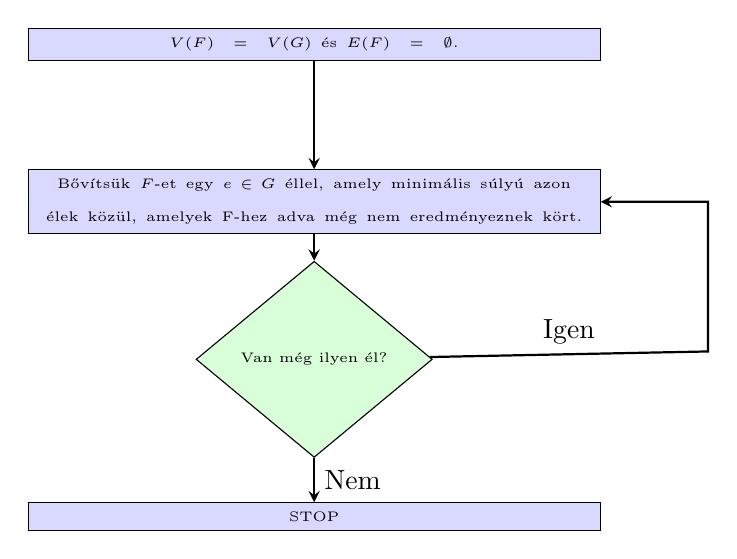
\begin{tikzpicture}[node distance = 2cm, auto]
    % Place nodes
    \node [block] (step1) {\tiny{$V(F)=V(G)$ és $E(F) = \emptyset$.}};
    \node [block, below of=step1] (step2) {\tiny{Bővítsük $F$-et egy $e \in G$ éllel, amely minimális súlyú azon élek közül, amelyek F-hez adva még nem eredményeznek kört.}};
    \node [decision, below of=step2] (step3) {\tiny{Van még ilyen él?}};
    \node [block, below of=step3] (step4) {\tiny{STOP}};

    \draw [arrow] (step1) -- (step2);
    \draw [arrow] (step2) -- (step3);
	\draw [arrow] (step3) -- node {Nem} (step4);    
    \draw[arrow] (step3) -- node {Igen} + (5, 0.1) |- (step2);
\end{tikzpicture}
\end{frame}

\begin{frame}
\begin{block}{Def.: Irányított gráf}

\end{block}
\end{frame}

\begin{frame}
\begin{block}{Tétel: Erős összefüggőség}
Egy összefüggő gráf akkor, és csak akkor irányítható úgy, hogy erősen összefüggő legyen, ha minden \textbf{éléhez} tartozik rajta áthaladó kör.
\end{block}
\end{frame}

\begin{frame}
\begin{block}{Tétel: Minimális fokszáma síkgráfban.}
Ha $G$ egyszerű, síkba rajzolható gráf, akkor $$\delta = \min_{{q \in V(G)}} d(a) \leq 5$$

\end{block}

\begin{block}{Bizonyítás (Indirekt)}
TFH $\delta \geq 6$.
Az általánosság megsértése nélkül feltehetjük, hogy $v(G) \geq 3$.\\
$\sum_{{a \in V(G)}} d(a) = 2e(G)$ (fokok száma = 2 x az élek száma)\\
Mivel $\delta \geq 6 \implies 6v(G) \leq 2e(G)$\\
A síkgráf élszáma tételből következik, hogy:\\
$2e(G) \leq 6v(G) - 12.$\\
\bigskip
$2e(G) \leq 6v(G) - 12$ \hspace{1ex} $/\cdot2$\\
$6v(G) \leq 6v(G) - 12$ $\rightarrow$ Ellentmondás!

\end{block}

\end{frame}

\begin{frame}
\begin{block}{Tétel: Kuratovski gráfok}
A Kuratovski gráfok ($K_5$ és $K_{3,3}$) Nem rajzolhatók síkba.\\
TODO: kép

\end{block}

\begin{block}{Bizonyítás (Indirekt)}
TFH $K_5$ és $K_{3,3}$ síkbarajzolható.\\
\smallskip
\textbf{$K_{3,3}$ esetén}:\\
$v(G) = 6$, és $e(G) = 9$\\
Euler forumlából következik, hogy $t = 5$.\\
Viszont $K_{3,3}$ nem tartalmaz háromszöget, és nincs szeparáló éle. $\implies$\\
$\implies$ $4t \leq 2e(G) \implies 20 \leq 18$. $\rightarrow$ Ellentmondás!\\
\smallskip
\textbf{$K_5$ esetén}:\\
$v(G) = 5$ és $e(G) = 10$\\
Alkalmazzuk a síkgráf élszáma tételt ($e(G) \leq 3v(G) - 6$), ekkor\\
$10 \leq 9$ $\rightarrow$ Ellentmondás!

\end{block}

\end{frame}

\begin{frame}
\begin{block}{Tétel: Kuratovski tétel}
Egy egyszerű véges gráf \textbf{akkor, és csak akkor} rajzolható síkba, ha nem tartalmaz a Kuratovski gráfok valamelyikével topologikusan izomorf részgráfot.

\end{block}

\end{frame}

\begin{frame}

\begin{block}{Tétel: Euler formula}
Egy összefüggő síkbeli gráf, amelynek $t$ tartománya van, (a külső tartományt is beleértve), eleget tesz az Euler-formulának:
$$v(G) - e(G) + t = 2$$

\end{block}

\begin{block}{Bizonyítás (Sematikus)}
Tekintsünk egy $K$ kört $G$-ben és egy $e \in E(K)$ élet.\\
Mivel $e$ két tartomány határán van $\implies$ $e$ törlésével két szomszéd régió eggyé válik.

(kép)

$\implies$ az élek, és tartományok száma is eggyel csökken.\\
A formula: $v(G) - e(G) + t = 2$ $\rightarrow$ $e(G)$ Az $e(G)$ nél ha kivonunk 1-et: $-(-1) = +1$, A $t$-nél pedig -1 $\implies$ a formula értéke ugyan az marad.\\

Az eltörléseket ismételve előbb-utóbb megkapjuk G egy feszítőfáját. (Tétel, feszítőfa létezése)

Fánál $t = 1$ és az élek száma $v(G) - 1$. $\implies$
$$\implies v(G) - e(G) + t = v(G) - (v(G) - 1) + 1 = 2$$

\end{block}
\end{frame}

\begin{frame}
\begin{block}{Tétel: Síkgráf élszáma}
 Ha $G$ egyszerű, síkba rajzolható gráf, és $v(G) \geq 3$, akkor $$e(G) \leq 3v(G) - 6$$.

\end{block}

\begin{block}{Bizonyítás}
\textbf{1. Eset}\\
TFH $G$ összefüggő.\\
Mivel $v(G) = 3$-ra igaz, ezért tfh (legyen) v(G) > 3.\\
Mivel G egyszeű $\implies$ minden tartományát legalább 3 él határolja. $\implies$\\
$\implies$ legalább 3t élet számoltunk.\\
Mivel az elvágó éleket egyszer számoltuk, a többit kétszer $\implies$ $3t \leq 2e(G)$.\\
Az Euler formulából következik, hogy $$3(e(G) - v(G) + 2) \leq 2e(G) \implies e(G) \leq 3v(G) - 6$$\\
\smallskip
\textbf{2. Eset}\\
TFH $G$ nem összefüggő.\\
Ekkor visszavezetjük az első esetre, élek hozzáadásával.

\end{block}

\end{frame}


% --------------------  FORÁLIS NYELVEK, ÉS AUTOMATÁK --------------------

\begin{frame}[plain]
\begin{beamercolorbox}[center]{title}
    {\Huge Formális nyelvek, és Automaták}
\end{beamercolorbox}
\end{frame}


\begin{frame}
\begin{block}{Def.: $\Sigma$ feletti szó}
Legyen $\Sigma$ véges nemüres halmaz.\\
\medskip
\textbf{$\Sigma$ feletti szón} a $\Sigma$ elemeiből (betűiből) képzett véges sorozatot értjük: \\
\medskip
$w = w_1 ... w_n$, $w_1 \in {\Sigma}, i = 1, ..., n$\\
\medskip
\textbf{Szó hossza:} Az $n$ nemnegatív, egész szám a w szó hossza. Jelölés: $|w|$.\\
($|w|_0$ a $w$-ben található $0$-k száma.)\\
\medskip
\textbf{Üres szó:} A $0$ hosszúságú szó, jelölése : $\epsilon$\\
\medskip
${\Sigma}^*$ jelöli a $\Sigma$ feletti szavak halmazát.\\
(Végtelen, viszont a szavak végesek)
\end{block}

\begin{block}{Def.: $\Sigma$ feletti nyelv}
${\Sigma}^*$ egy részhalmazát \textbf{$\Sigma$ feletti nyelvnek} nevezzük.
\end{block}

\begin{block}{Def.: Véges automata}
\textbf{$(Q, {\Sigma}, {\delta}, q_0, F)$}\\
\medskip
$Q$: Állapotok véges, nemüres halmaza.\\
\medskip
$\Sigma$: bemenő jelek (betűk) véges, nemüres halmaza.\\
\medskip
$\delta : Q x \Sigma \rightarrow Q$: átmeneti függvény.\\
\medskip
$q_0 \in Q$: Kezdőállapot.\\
\medskip
$F \subseteq Q$: Végállapotok halmaza.\\
\end{block}

\end{frame}

\begin{frame}
\begin{block}{Def.: Számítási sorozat, elfogadott szó, felismert nyelv}
Legyen $M = (Q, {\Sigma}, {\delta}, q_0, F)$ véges automata, $q \in Q$ és $w = w_1...w_n \in {\Sigma}^*$, ekkor az\\
\medskip
$r_0, r_1, ..., r_n (r_i \in Q, i = 1, ..., n)$\\
\medskip
állapotsorozat az $M$ $q$-ból induló számítási sorozata a $w$ szón, ha\\
\medskip
$r_0 = q$ és $r_i = {\delta}(r_{i - 1}, w_i)(i = 1, ..., n)$\\
\bigskip
\textbf{Elfogadott szó:} Azt mondjuk, hogy \textbf{$M$ elfogadja a $w$ szót}, ha létezik a $q_0$ kezdőállapotból induló számítási sorozat a $w$ szón és $r_n \in F$.\\
\bigskip
\textbf{Felismert nyelv:} Az M által felismert nyelv: $L(M) = \{w \in {\Sigma}^* | M$ elfogadja $w$-t$\}$.\\
\bigskip
Két automata \textbf{ekvivalens}, ha ugyanazt a nyelvet ismerik fel.
\end{block}

\begin{block}{Def.: Felismerhető nyelv}
Az $L \subseteq {\Sigma}^*$ nyelvet \textbf{felismerhető nyelvnek} nevezzük, ha létezik olyan véges automata, amely felismeri.
\end{block}

\begin{block}{Def.: Konkatenáció}
$A$ $\cdot : {\Sigma}^* x {\Sigma}^* \rightarrow {\Sigma}^*$ műveletet konkatenációnak nevezzük, ahol\\
\medskip
$u, v \in {\Sigma}^*, u = u_1...u_n, v = v_1...v_n$ esetén\\
$u \cdot v = u1...u_nv_1...v_n$
\end{block}

\begin{block}{Ész}
$({\Sigma}^*, {\cdot})$ egységelemes félcsoport (monoid).\\
\begin{enumerate}
\item $\cdot$ zárt, mivel $u \cdot v = u_1...u_nv_1...v_n \in {\Sigma}^*$.
\item Asszociatív: $(u \cdot v) \cdot w = u \cdot (v \cdot w)$.
\item $\epsilon$ egységelem: $u \cdot \epsilon = \epsilon \cdot u = u$.
\end{enumerate}
\end{block}

\end{frame}

\begin{frame}
\begin{block}{Def.: Egyesítés,Metszet, Komplementer, Konkatenáció, Iteráció}
Legyen $L, L_1, L_2 \subseteq {\Sigma}^*$, ekkor\\
\medskip
\begin{enumerate}
\item $L_1 \cup L_2 = \{v \in {\Sigma}^* : v \in L_1 \lor v \in L_2\}$ (Egyesítés) (Reguláris művelet)
\item $L_1 \cap L_2 = \{v \in {\Sigma}^* : v \in L_1 \land v \in L_2\}$ (Metszet)
\item $\overline{L} = \{v \in {\Sigma}^* : v \notin L\}$ (Komplementer)
\item $L_1 \cdot  L_2 = \{uv : v \in L_1 \land u \in L_2\}$ (Konkatenáció) (Reguláris művelet)\\
Nem kommutatív! ($L_1$ $=$ $\{$alma, fűz$\}$, $L_2$ $=$ $\{$fa$\}$, $L_1 \cdot L_2$ $=$ $\{$almafa, fűzfa$\}$, de fordítva nem!) (Minden elemet minden elemmel, úgy, hogy a sorrend számít!)
\item $L^* = \{v_1...v_n : n \geq 0, v_1, ..., v_n \in L\}$ (Iteráció) (Reguláris művelet)\\
(Klíni-féle iteráció) (Összes lehetséges módon képezzük, + $\epsilon$)
\end{enumerate}
\end{block}

\end{frame}

\begin{frame}
\begin{block}{Műveleti azonosságok}
$L_1 \cup (L_2 \cup L_3) = (L_1 \cup L_2) \cup L_3$\\
$L_1 \cup L_2 = L_2  \cup L_1$\\
$L \cup L = L$\\
$L \cup \emptyset = L$\\
\bigskip
$L_1 \cdot (L_2 \cdot L_3) = (L_1 \cdot L_2) \cdot L_3$\\
$L \cdot \{{\epsilon}\} = L$\\
$\{{\epsilon}\} \cdot L = L$\\
$L \cdot \emptyset = \emptyset$\\
$\emptyset \cdot L = \emptyset$\\
\bigskip
$L_1 \cdot (L_2 \cup L_3) = (L_1 \cdot L_2) \cup (L_1 \cdot L_3)$\\
$(L_1 \cup L_2) \cdot L_3 = (L_1 \cdot L_3) \cup (L_2 \cdot L_3)$\\
\bigskip
Jelölések:\\
\medskip
$L^+ = L \cdot L^* = L^* \cdot L$\\
$L^n = L \cdot ... \cdot L$ ($n$-szer), $L^0 = \{{\epsilon}\}$\\
\medskip
Észrevétel:\\
\medskip
$L^* = \bigcup_{n \geq 0} L^n$\\
$L^+ = \bigcup_{n \geq 1} L^n$\\
\smallskip
Tehát: $L^* = L^+ \cup \{{\epsilon}\}$
\end{block}

\end{frame}

\begin{frame}

\begin{block}{Def.: Reguláris nyelv}
Az $L \subseteq {\Sigma}^*$ nyelvet \textbf{reguláris nyelvnek} nevezzük, ha előáll az\\
$\emptyset$ és $\{a\}$ $(a \in {\Sigma})$\\
nyelvekből a három reguláris művelet véges sokszori alkalmazásával.
\end{block}

\begin{block}{Tétel: Kleene tétel}
Egy nyelv akkor, és csak akkor felismerhető, ha reguláris.
\end{block}

\end{frame}

\begin{frame}
\begin{block}{Tétel: Felismerhető nyelvek komplementere}
$L$ Felismerhető $\implies$ $\overline{L}$

\end{block}

\begin{block}{Bizonyítás}
Legyen $M = (Q, \Sigma , \delta , q_0, F)$ véges automata és $L = L(M)$ (M automata felismeri az L nyelvet).\\
Tekintsük a következő konstrukciót:\\
Legyen $\overline{M} = (Q, \Sigma , \delta, q_0, \overline{L})$, ahol $\overline{F} = Q - F$.\\
Ekkor  $L(\overline{M}) = \overline{L}$. (Azaz az $\overline{M}$ automata biztosan felismeri az $\overline{L}$ nyelvet.\\ 
(Triviális, mert amit $L$ nem ismer fel, azt ez biztosan, amit $\overline{L}$ felismer, azt pedig ez nem ismeri fel biztosan.

\end{block}

\end{frame}

\begin{frame}
\begin{block}{Tétel: Felismerhető nyelvek metszete}
$L_1, L_2$ felismerhető $\implies$ $L_1 \cap L_2$

\end{block}

\begin{block}{Bizonyítás}
Legyen: $L_1 = L(M_1), L_2 = L(M_2)$.\\
Legyen: $M_1 = (Q_1, \Sigma , {\delta}_1, q_1, F_1), M_2 = (Q_2, \Sigma , {\delta}_2, q_2, F_2)$.\\
Legyen: $Q = Q_1 x Q_2$ (Párokból áll, ha pl $Q_1$ 2 elemű, $Q_2$ 3 elemű, akkor $Q$ 6 elemből fog állni.)\\
Legyen: $\delta = Q x \Sigma \rightarrow Q$ (Párok lesznek).\\
Legyen: $\delta(s, a), s \in Q = \delta((s_1, s_2), a) = ({\delta}_1(s_1, a), {\delta}_2(s_2, a))$, $s_1 \in Q_1, s_2 \in Q_2, a \in \Sigma$\\
\bigskip
Legyen: $q_0 = (q_1, q_2)$\\
Legyen: \underline{\textbf{$F_{\cap} = F_1 x F_2$}} (Az összes lehetséges módon párokat képzünk mindkét alap automata végállapot halmazaiból) $\implies$ csak akkor fog egy nyelvet felismerni, a "nagy" automata, ha mindkét "kis" automata az egyik eredeti végállapotában áll.)\\
\smallskip
Legyen: $M_{\cap} = (Q, \Sigma , \delta , q_0, F_{\cap})$\\
\bigskip
Ekkor: \underline{$L(M_{\cap}) = L_1 \cap L_2$}\\
\end{block}

\end{frame}

\begin{frame}
\begin{block}{Tétel: Felismerhető nyelvek egyesítése}
$L_1, L_2$ felismerhető $\implies$ $L_1 \cup L_2$

\end{block}

\begin{block}{Bizonyítás}
Legyen: $L_1 = L(M_1), L_2 = L(M_2)$.\\
Legyen: $M_1 = (Q_1, \Sigma , {\delta}_1, q_1, F_1), M_2 = (Q_2, \Sigma , {\delta}_2, q_2, F_2)$.\\
Legyen: $Q = Q_1 x Q_2$
Legyen: $\delta = Q x \Sigma \rightarrow Q$ (Párok lesznek).\\
Legyen: $\delta((s_1, s_2), a) = ({\delta}_1(s_1, a), {\delta}_2(s_2, a))$, $s_1 \in Q_1, s_2 \in Q_2, a \in \Sigma$\\
\bigskip
Legyen: $q_0 = (q_1, q_2)$\\
Legyen: \underline{\textbf{$F_{\cup} = F_1 x Q_2 \cup F_2 x Q_1$}} (Az \textbf{első} "kicsi" automata összes \textbf{végállapotát} párba vesszük a \textbf{második} "kicsi" automata összes \textbf{állapotával}, unió a \textbf{második} "kicsi" automata összes végállapota az első "kicsi" automata \textbf{állapotával} $\implies$ bármelyik "kicsi" automata végállapotba kerül, az a másiknak is végállapota lesz a pár másik felén. (Mivel pároknál számít az elemek sorrendje))\\
\smallskip
Legyen: $M_{\cup} = (Q, \Sigma , \delta , q_0, F_{\cup})$\\
\bigskip
Ekkor: \underline{$L(M_{\cup}) = L_1 \cup L_2$}\\
\end{block}

\end{frame}

\begin{frame}
\begin{block}{Def.: Nemdeterminisztikus automata}
\textbf{Véges nemdeterminisztikus (üres átmenetekkel ellátott) automata:}\\
\medskip
$M = (Q, {\Sigma}, {\delta}, q_0, F)$,\\
\medskip
ahol $Q, {\Sigma}, q_0, F$ ugyanazok, mint véges automatában, továbbá:\\
\medskip
$\delta : Q$ $x$ $({\Sigma} \cup \{{\epsilon}\}) \rightarrow p(Q)$
\end{block}

\begin{block}{Def.: Számítási sorozat, elfogadott szó, felismert nyelv}
Legyen $M = (Q, {\Sigma}, {\delta}, q_0, F)$ véges \underline{nemdeterminisztikus} automata, $q \in Q$ és \underline{$w \in {\Sigma}^*$}, ekkor az\\
\medskip
$r_0, r_1, ..., r_n (r_i \in Q, i = 1, ..., n)$\\
\medskip
állapotsorozat az $M$ $q$-ból induló számítási sorozata a $w$ szón, ha \underline{$w$ felírható}\\
\medskip
\underline{$w = w_1 ... w_n, w_i \in {\Sigma}_{\epsilon}, (i = 1, ..., n)$}\\
\medskip
\underline{alakban úgy, hogy:}\\
\medskip
$r_0 = q$ és $r_i = {\delta}(r_{i - 1}, w_i)(i = 1, ..., n)$\\
\bigskip
\textbf{Elfogadott szó:} Azt mondjuk, hogy \textbf{$M$ elfogadja a $w$ szót}, ha létezik a $q_0$ kezdőállapotból induló számítási sorozat a $w$ szón és $r_n \in F$.\\
\bigskip
\textbf{Felismert nyelv:} Az M által felismert nyelv: $L(M) = \{w \in {\Sigma}^* | M$ elfogadja $w$-t$\}$.\\
\bigskip
(az aláhúzotta különböznek a determinisztikus automatáshoz képest)
\end{block}

\begin{block}{Def.: $X \epsilon$-lezártja}
Legyen $X \subseteq Q$. Ekkor \textbf{$X \epsilon$-lezártján} s állapotok olyan $\widehat{X}$ halmazát értjük, amelyekre létezik $X$-beli $q$ állapotból induló számítási sorozat az $\epsilon$ szón, amely $s$-ben végződik.\\
Formalizálva:\\
$\widehat{X} = \{s \in Q : {\exists}r_0,r_1,...,r_n, n \geq 0, r_0 \in X, r_n = s, r_i \in {\delta}(r_{i - 1}, {\epsilon}), i = 1, ..., n\}$.\\
{\tiny (S) Azaz ha egy számítási sorozat végéből átmenet van csak $\epsilon$-al, akkor hozzávesszük azokat is, ameddig szükséges, és az első nem $\epsilon$-os átmenet lessza vége.}\\
{\tiny (S) A definíció listában nincs benne, de az egyik bizonyításban fel van használva}
\end{block}
\end{frame}

\begin{frame}
\begin{block}{Tétel: Nemdeterminisztikus automata}
Minden $M = (Q, \Sigma , \delta , q_0, F)$ véges nemdeterminisztikus automatával felismerhető nyelv, felismerhető véges automatával.
\end{block}

\begin{block}{Bizonyítás}
Tekintsük az $M' = (Q', \Sigma , {\delta}', Q_0, F')$ véges automatát ($Q_0$ halmaz!), ahol\\
$Q' = p(Q)$ ($p(Q)$ $\rightarrow$ hatványhalmaz)\\
${\delta}' : p(Q) x \Sigma \rightarrow p(Q)$ (Az állapotok is halmazok!)\\
${\delta}'(X, a) = \widehat{Y}$ (Y lezártja!), $Y = U_{q \in X} \delta(q, a)$\\
$Q_0 = \widehat{\{q_0\}}$\\
$F' = \{X \subseteq Q : X \cap F \neq \emptyset \}$.\\
Ekkor nyilvánvaló, hogy $L(M') = L(M)$.\\
Megjegyzés: Elég lenne $p(Q)$ azon elemeivel számolni, amelyek elérhetők $Q_0$-ból.

\end{block}

\end{frame}

\begin{frame}
\begin{block}{Tétel: Felismerhető nyelvek szorzata}
$L_1, L_2$ felismerhető $\implies$ $L_1 \cdot L_2$

\end{block}

\begin{block}{Bizonyítás}
Legyen: $L_1 = L(M_1), L_2 = L(M_2)$.\\
Legyen: $M_1 = (Q_1, \Sigma , {\delta}_1, q_1, F_1), M_2 = (Q_2, \Sigma , {\delta}_2, q_2, F_2)$.\\
Legyen: $Q_1 \cap Q_2 = \emptyset$\\
Legyen: $L(M_1) = L_1, L(M_2) = L_2$.\\
\bigskip
Legyen: ${\delta}(q, a) = $
$
\begin{cases}
{\delta}_1(q, a) & q \in Q_1 - F_1\\
{\delta}_1(q, a) & q \in F_1, a \neq \epsilon $ (Végállapot) $\\
{\delta}_1(q, a) \cup \{q_2\} & q \in F_1, a = \epsilon $ (Végállapot) $\rightarrow \\
 & \rightarrow$ Ha üres betű, akkor átugrunk a második automata kezdőállapotába.$\\
{\delta}_2(q, a) & q \in Q_2 $ A második automata $ \\
\end{cases}
$\\
\bigskip
Legyen: $M_1 \cdot M_2 = (Q_1 \cup Q_2, \Sigma , \delta , q_1, F_2)$\\
\bigskip
Ekkor: \textbf{$L(M_1 \cdot M_2) = L_1 \cdot L_2$}\\
\end{block}

\end{frame}

\begin{frame}
\begin{block}{Tétel: Felismerhető nyelvek iterációja}
$L$ felismerhető $\implies$ $L^*$ is felismerhető.

\end{block}

\begin{block}{Bizonyítás}
Legyen: $M = (Q, \Sigma , {\delta}, q_0, F)$.\\
Legyen: $M^* = (Q \cup \{s_0\}, \Sigma , {\delta}_*, s_0, F \cup \{s_0\})$.\\
\bigskip
Legyen: ${\delta}(q, a)_* = $
$
\begin{cases}
{\delta}(q, a) & q \in Q $ és $q \notin F\\
{\delta}(q, a) & q \in F$ és $a \neq \epsilon \\
{\delta}(q, a) \cup \{q0\} & q \in F$ és $a = \epsilon \\
\{q_0\} & q = s_0$ és $a = \epsilon \\
\emptyset & q = s_0$ és $a \neq \epsilon \\
\end{cases}
$\\
\bigskip
\textbf{Ekkor: $L(M^*) = L^*$}\\
\end{block}

\end{frame}
\begin{frame}
\begin{block}{Def.: Reguláris kifejezések}
$\Sigma$ véges, nemüres halmaz.\\
Azt mondjuk, hogy $R$ reguláris kifejezés ($\Sigma$ felett), ha:\\
\medskip
\begin{enumerate}
\item $R = a$  valamely $a \in \Sigma$-ra, és ekkor $R$ a $\{a\}$ nyelvet jelöli, vagy
\item $R = \emptyset$ és ekkor $R$ az $\emptyset$ nyelvet jelöli, vagy
\item $R = (R_1 + R_2)$ és ekkor $R$ az $R_1$ és $R_2$ által jelölt nyelvek egyesítését jelöli, vagy
\item $R = (R_1 \cdot R_2)$ és ekkor $R$ az $R_1$ és $R_2$ által jelölt nyelvek konkatenációját jelöli, vagy
\item $R = (R^*_1)$ és ekkor az $R$ az $R_1$ által jelölt nyelv iterációját jelöli.
\end{enumerate}
\medskip
ahol $R_1, R_2$ reguláris kifejezések.
\end{block}
\end{frame}

\begin{frame}
\begin{block}{Tétel: Pumpáló lemma reguláris nyelvre}
Minden $L \subseteq {\Sigma}^*$ reguláris nyelvhez létezik olyan $p$ természetes szám, amelyre L minden legalább $p$ hosszúságú $u$ szava felírható $$u = xyz$$\\
alakban úgy, hogy\\
\begin{enumerate}
\item $|y| > 0$
\item $|xy| \leq p$
\item $xy'z \in L$ minden $i \geq 0$ egészre.
\end{enumerate}

\end{block}

\begin{block}{Bizonyítás}
Az L reguláris nyelvhez konstruáljuk meg az $M = (Q, {\Sigma}, {\delta}, q_0, F)$ véges automatát úgy, hogy legyen $p = |Q|$.\\
Ha $u \in L$ és $|u| \geq p \implies$ a $q_0, q_1, ...,q_n (q_i \in Q, i = 0, ..., n)$\\
számítási sorozatra az $u$ szón teljesüljön, hogy\\
\begin{enumerate}
\item $n = |u| \geq p$
\item $q_n \in F$
\item ${\exists}i, j : 0 \leq i < j \leq p$ és $q_i = q_j$
\end{enumerate}
\bigskip
Legyen továbbá:
\begin{itemize}
\item $x$ az $u$ szó $i$ hosszú kezdőszelete
\item $y$ az $x$-et követő $j - i$ hosszú rész-szó
\item $z$ az $u$-nak az $n - j$ hosszú zárószelete 
\end{itemize}
\bigskip
\textbf{Ekkor az $u = xyz$ felbontásra teljesülnek a lemma állításai.}
\end{block}

\end{frame}

\begin{frame}
\begin{block}{Tétel: Példa nemreguláris nyelvre}
Az $L = \{0^n1^n : n \geq 0\} \subseteq \{0, 1\}^*$ nyelv nem reguláris.
\end{block}

\begin{block}{Bizonyítás}
Legyen $p$  tetszőleges, ekkor $u$ (szó) $ = 0^p1^p$.\\
Tfh $x, y, z$ olyan szavak, amelyekre:\\
$u = xyz, |xy| \leq p, |y| > 0$.\\
\bigskip
Ekkor $xy$ csupa 0-ból áll és $y$ tartalmaz legalább egy 0-t. $\implies$\\
$\implies$ $i \neq 1$ esetén $xy'z \notin L$, mert több 0 lessz benne, mint 1-es! $\implies$\\
$\implies$ Sosem találunk megfelelő $p$-t $\implies$ \textbf{A nyelv nem reguláris.}\\
\bigskip
TODO: Példa értékek
\end{block}

\end{frame}

\begin{frame}
\begin{block}{Def.: Környezetfüggetlen nyelvtan}
\textbf{Környezetfüggetlen nyelvtannak} nevezzük a\\
$G = (V, {\Sigma}, R, S)$ négyest, ahol\\
\begin{itemize}
\item $V$ véges, nemüres halmaz: a változók vagy nemterminálisok abc-je
\item $\Sigma$ véges, nemüres halmaz: a terminálisok abc-je, ahol $V \cap \Sigma = \emptyset$ (Betűk)
\item $R : A \rightarrow w$ alakú átírási szabályok véges halmaza, ahol $A \in V, w \in (V \cup {\Sigma})^*$\\
(Nem terminálisokhoz hozzárendelünk terminális szimbólumokat.), (Nem biztos, hogy terminális), ($A$ helyettesíthető a $w$-vel minden esetben.), ($w$ $\rightarrow$ lehetnek végtelen hosszú szavak.)
\item $S \in V$ a kezdőszimbólum.
\end{itemize}
\end{block}

\begin{block}{Def.: Deriváció, közvetlen derivált}
Legyen $G = (V, {\Sigma}, R, S)$ környezetfüggetlen nyelvtan, $u, v \in (V \cup {\Sigma})^*$.\\
\medskip
\textbf{Közvetlen derivált:}\\
Azt mondjuk, hogy \textbf{$u$ közvetlen deriváltja a $v$ szó}, Jelölés: $u \Rightarrow v$,\\
ha létezik az $u = u_1Au_2$ és $v = u_1wu_2$ felbontás úgy, hogy $A  \rightarrow w \in R$.\\
\medskip
\textbf{$v$ szó $u$ ból való derivációja:}\\
Egy $u_0, u_1, ..., u_n (n \geq 0)$ sorozatot a \textbf{$v$ szó $u$-ból való derivációjának} nevezünk, ha:\\
$u_0 = u, u_n = v$ és\\
$u_{i - 1} \Rightarrow u_i, i = 1, ..., n$.\\
\medskip
\textbf{Levezethető:}\\
Azt mondjuk, hogy a \textbf{$v$ deriválható vagy levezethető $u$-ból},
\\ha létezik a $v$-nek $u$-ból való derivációja.\\
Jele: $u {\Rightarrow}^* v$.\\
\medskip
A \textbf{$G$ által generált nyelv}:\\
$L(G) = \{w \in {\Sigma}^* : S {\Rightarrow}^* w\}$.

\end{block}

\begin{block}{Def.: Nyelvtanok ekvivalenciája, Környezetfüggetlen nyelv}
Két nyelvtan \textbf{ekvivalens}, ha ugyanazt a nyelvet generálják.\\
Egy nyelv \textbf{Környezetfüggetlen}, ha generálható környezetfüggetlen nyelvtannal.
\end{block}

\end{frame}

\begin{frame}
\begin{block}{Def.: Derivációs fa}
Legyen $G = (V, {\Sigma}, R, S)$ környezetfüggetlen nyelvtan.\\
\textbf{$G$ feletti derivációs fa} olyan véges, irányított, rendezett fa, amely csúcsai a $V \cup {\Sigma} \cup \{{\epsilon}\}$ halmaz elemeive címkézettek úgy, hogy valahányszor egy csúcs és leszármazottainak címét rendre\\
\medskip
$X, X_1, ..., X_n (n \geq 1)$,\\
mindannyiszor $X \rightarrow X_1...X_n \in R$.\\
\medskip
Továbbá minden levél címkéje az $\{{\epsilon}\} \cup {\Sigma} = {\Sigma}_g$ halmazban van, és ha egy csúcs valamely leszármazottja $\epsilon$-nal címkézett, akkor a csúcsnak egyetlen leszármazottja van.\\
\bigskip
Ha a gyökér címkéje $X$, akkor a \textbf{derivációs fa $X$-ből indul}.\\
\bigskip
A derivációs fa leveleinek, illetve a levelek címkéinek sorozata a \textbf{derivációs fa határa}, amely egy ${\Sigma}^*$-beli szó.
\end{block}
\end{frame}

\begin{frame}
\begin{block}{Tétel: Derivációs fák}
Egy $X \in (V \cup {\Sigma}_{\epsilon})$-ből induló derivációs fa, amelynek határa az $u \in {\Sigma}^*$ szó, ami akkor és csak akkor létezik, ha $X {\Rightarrow}^* u \in {\Sigma}^*$.
\end{block}

\begin{block}{Def.: Jobb-, Baloldali deriváció}
Azt mondjuk, hogy egy\\
\bigskip
$u_0 \Rightarrow u_1 \Rightarrow ... \Rightarrow u_n$\\
\bigskip
\textbf{deriváció baloldali}, ha minden $i < n$ számra $u_{i + 1}$ úgy áll elő az $u_i$ szóból, hogy az $u_i$-ben előforduló első nemterminálist írjuk át.\\
\bigskip
\textbf{Jobboldali derivációk} hasonlóan definiálhatóak.\\
\bigskip
Baloldali deriváció jelölése:\\
\bigskip
$u_0 {\Rightarrow}_l ... {\Rightarrow}_l u_g$, vagy $u_0 {\Rightarrow}^*_l u_g$.
\end{block}
\end{frame}

\begin{frame}
\begin{block}{Tétel: Ekvivalens állítások derivációs fákra}
Legyen $G = (V, {\Sigma}, R, S)$ környezetfüggetlen nyelvtan. Ekkor a következők ekvivalensek az $u \in {\Sigma}^*$ szóra:\\
\begin{enumerate}
\item $u \in L(G)$
\item $S {{\Rightarrow}^*}_l u$
\item Létezik olyan $S$-ből induló derivációs fa, amelynek határa $u$.
\end{enumerate}
\end{block}

\end{frame}

\begin{frame}
\begin{block}{Egyértelmű nyelvtan}
A $G = (V, {\Sigma}, R, S)$ \textbf{nyelvtant egyértelműnek} nevezzük, ha minden $u \in L(G)$ szónak pontosan egy $S$-ből induló baloldali levezetése (derivációs fája) van.
\end{block}
\end{frame}

\begin{frame}
\begin{block}{Tétel: Reguláris nyelv környezetfüggetlen}
Minden reguláris nyelv környezetfüggetlen.
\end{block}

\begin{block}{Bizonyítás (Konstr)}
Legyen $L \in {\Sigma}^*, L = L(M)$, és\\
$M = (Q, {\Sigma}, {\delta}, q_0, F)$ nemdeterminisztikus véges automata.\\
\bigskip
Megkonstruáljuk a $G = (Q, {\Sigma}, R, q_0)$ nyelvtant, ahol,\\
$R = \{q \rightarrow aq' : q' \in {\delta}(q, a)\} \cup \{q \rightarrow \epsilon : q \in F \}$.\\
Ekkor az $u \in  L(G) \iff \exists u$ szóra $q_0$-ból $q$-ba vezető számítási sorozat.\\
(triviális, a vizsgán is lehet mondani).
\end{block}

\end{frame}

\begin{frame}
\begin{block}{Jobblineáris nyelvtan, nyelv}
A $G = (V, {\Sigma}, R, S)$ környezetfüggetlen \textbf{nyelvtan jobblineáris},\\
Ha minden osztálya:\\
\medskip
$A \rightarrow uB$ vagy $A \rightarrow u$ alakú, ahol $u \in {\Sigma}^*$ és $A, B \in V$\\
\bigskip
L \textbf{nyelv jobblineáris}, ha generálhatü jobblineáris nyelvtannal.\\
\smallskip
(Ez a legszigorúbb szabály, a reguláris nyelveket tudja generálni.)
\end{block}
\end{frame}

\begin{frame}
\begin{block}{Tétel: Környezetfüggetlen nyelvek műveleti zártsága}
A környezetfüggetlen nyelvek zártak a reguláris műveletekre.
\end{block}

\begin{block}{Bizonyítás (Kontrapozíció)}
A módszer: adott $E$ reguláris kifejezéshez megadjuk a\\
$G_E = (V_E, {\Sigma}, R_E, S_E)$\\
nyelvtant, amely az $E$ által jelölt nyelvet generálja.\\
\bigskip
Legyen először $E = \emptyset$:\\
Akkor $G_{\emptyset} = (\{S\}, {\Sigma}, \emptyset, S)$.\\
\bigskip
Ha $E = a \in {\Sigma}$:\\
Akkor $G_a = (\{S\}, {\Sigma}, \{S \rightarrow a\}, S)$.\\
\bigskip
Ha $E = (E_1 + E_2)$:\\
Akkor $G_E = (V_{E_1} \cup V_{E_2} \cup \{S\}, \Sigma, R_{E_1} \cup R_{E_2} \cup \{S \rightarrow S_{E_1}, S \rightarrow S_{E_2}\}, S)$,\\
és feltesszük, hogy $V_{E_1} \cap V_{E_2} = {\emptyset}, S \notin V_{E_1} \cup V_{E_2}$.\\
\bigskip
Ha $E = (E_1 \cdot E_2)$:\\
Akkor $G_E = (V_{E_1} \cup V_{E_2} \cup \{S\}, \Sigma, R_{E_1} \cup R_{E_2} \cup \{S \rightarrow S_{E_1}S_{E_2}\}, S)$,\\
és feltesszük, hogy $V_{E_1} \cap V_{E_2} = {\emptyset}, S \notin V_{E_1} \cup V_{E_2}$.\\
\bigskip
Ha $E = (E_1)^*$:\\
Akkor $G_E = (V_{E_1} \cup \{S\}, \Sigma, R_{E_1} \cup \{S \rightarrow SS_{E_1}, S \rightarrow \epsilon \}, S)$,\\
és feltesszük, hogy $S \notin V_{E_1}$.\\

\end{block}
\end{frame}

\begin{frame}
\begin{block}{Def.: Veremautomata, Elfgadott szó}
\textbf{Veremautomata} egy $M = (Q, {\Sigma}, {\Gamma}, {\delta}, q_0, F)$ rendszer,\\
ahol $Q, {\Sigma}, q_0, F$ ugyanazok, mint véges automata esetén, továbbá\\
\medskip
$\Gamma$ : véges, nemüres halmaz, a verem ábécé.\\
$\delta : Q x {\Sigma}_g x {\Gamma}_g \rightarrow p(Q x {\Gamma}_g)$ az átmenetfüggvény.\\
\bigskip
\textbf{Elfogadott szó:}\\
Az \textbf{$M$ veremautomata akkor fogadja el a $w \in {\Sigma}^*$ szót,} ha\\
${\exists}w_1, ..., w_m \in {\Sigma}_g, r_0, ..., r_m \in Q, s_0, ..., s_m \in {\Gamma}^*$, ahol\\
\begin{enumerate}
\item $w = w_1...w_m$\\
\item $r_0 = q_0, s_0 = \epsilon$
\item ${\forall}i < m (r_{i + 1}, b) \in {\delta}(r_i, w_{i + 1}, a)$, ahol $s_i = at$ és $s_{i + 1} = bt$\\
valamely $a, b \in {\Gamma}_g, t \in {\Gamma}^*$ esetén.
\item $r_m \in F$
\end{enumerate}
\medskip
Jelölés: $L(M)$ jelöli az $M$ által elfogadott $w \in {\Sigma}^*$ szavak halmazát.\\
$L(M)$-et am $M$ által felismert nyelvnek nevezzük.
\end{block}
\end{frame}

\begin{frame}
\begin{block}{Def.: Konfiguráció}
\textbf{Konfiguráció} a $(q, {\alpha}, u) \in Q x {\Sigma}_{\epsilon} x {\Gamma}_{\epsilon}$ rendezett hármas.\\
\medskip
$(q, {\alpha}, u) \vdash (q', {\alpha}', u')$,\\
{\tiny (S) A $\vdash$ kb levezethetőt jelent, de nem biztos, hogy ez a szakszó rá!}
\medskip
ha létezik olyan $((q, a, {\gamma}), (q', {\gamma}'))$ szabály és $\mathcal{B} \in {\Gamma}^*$, hogy\\
\medskip
$u = au'$, $\alpha = {\gamma}{\beta}$, ${\alpha}' = {\gamma}'{\beta}$.\\
\medskip
$(q, {\alpha}, u) {\vdash}^* (q', {\alpha}', u')$.\\
\medskip
ha valamely $(r_i, {\alpha}_i, u_i), i = 0, ..., n$ konfigurációkra\\
\medskip
$(r_0, {\alpha}_0, u_0) = (q, {\alpha}, u)$, $(r_n, {\alpha}_n, u_n) = (q', {\alpha}', u')$, és\\
$(r_i, {\alpha}_i, u_i) \vdash (r_{i + 1}, {\alpha}_{i + 1}, u_{i + 1})$ minden $i = 0, ..., n - 1$ esetén.\\
\end{block}
\end{frame}

\begin{frame}
\begin{block}{Tétel: Környezetfüggetlen nyelv és veremautomata}
Minden környezetfüggetlen nyelv felismerhető veremautomatával és minden veremautomatával felismerhető nyelv környezetfüggetlen.
\end{block}

\begin{block}{Tétel: Pumpáló lemma környezetfüggetlen nyelvre}
Minden $L \subseteq {\Sigma}^*$ környezetfüggetlen nyelvhez létezik olyan $p > 0$ természetes szám, amelyre L minden legalább $p$ hosszúságó $w$ szava felírható $$w = uvxyz$$\\
alakban úgy, hogy\\
\begin{enumerate}
\item $|vy| > 0$
\item $|vxy| < p$
\item $uv'xy'z \in L$ minden $i \geq 0$ egészre.
\end{enumerate}

\end{block}
\end{frame}

\begin{frame}
\begin{block}{Tétel: Példa nem környezetfüggetlen nyelvre 1}
Az $L = \{a^nb^nc^n : n \geq 0 \} \subseteq \{a, b, c\}^*$ nyelv nem környezetfüggetlen.
\end{block}

\begin{block}{Bizonyítás}
Belátjuk, hogy ${\forall}p > 0$ egészhez ${\exists}w \in L, |w| \geq p$ úgy, hogy\\
a $w$ tetszőleges olyan $w = uvxyz$ felbontására, ahol $|vy| > 0, |vxy| < p$,\\
létezik olyan i, amelyre $uv^ixy^iz \notin L$.\\
\bigskip
Tetszőleges $p$-hez legyen $w = a^pb^pc^p$. Ekkor bárhogyan is írjuk fel a $w$-t úgy, hogy $w = uvxyz$ felbontásra $|vy| > 0, |vxy| < p$, mindíg lesz olyan betű, amely nincs benne $vy$-ban, viszont ekkor $uxz \notin L$.
\end{block}
\end{frame}

\begin{frame}
\begin{block}{Tétel: Példa nem környezetfüggetlen nyelvre 2}
Az $L = \{w\#w : w \in \{0, 1\}^* \}$ nyelv nem környezetfüggetlen.
\end{block}

\begin{block}{Bizonyítás}
Tetszőleges $p$-hez legyen $w = 0^p1^p\#0^p1^p$, és tekintsük $w$ egy tetszőleges olyan $w = uvxyz$ felbontását, ahol $|vy| > 0, |vxy| < p$.\\
\bigskip
1. eset: Ha $\# \notin x$ $\rightarrow$ $uv^2xy^2z \notin L$.\\
\bigskip
2. eset: Ha $\# \in x$ $\rightarrow$ Ekkor $u$-ban csak az $1, y$-ban csak $0$ szerepelhet. $\rightarrow$ Mivel $vy \neq \epsilon \Rightarrow uxz \notin L$.
\end{block}
\end{frame}

\end{document}
